\documentclass[12pt]{article}
\usepackage{makeidx}
\makeindex
\usepackage{subcaption}
\usepackage[utf8]{inputenc}%acentuação das palavras
\usepackage[T1]{fontenc}%codificação de fonte
\usepackage[brazilian]{babel}
\usepackage{tikz}
\usepackage{textcomp}
\usepackage{afterpage}
\usepackage{varwidth}
\usepackage{indentfirst}
\usepackage{amsfonts}
\usepackage{amsmath}
\usepackage{amsthm}
%\usepackage{amssymb}
\usepackage{amscd}
\usepackage{amsxtra}
\usepackage{latexsym}
\usepackage{hyperref}
%\usepackage{cleveref}
\usepackage{enumerate}
\usepackage{fancyhdr}
\usepackage{etoolbox}
\usepackage{multicol}
\usepackage{multirow}
\usepackage{setspace} \onehalfspacing
\usepackage{mathptmx}
\usepackage[portuguese,ruled,vlined,linesnumbered]{algorithm2e}%algoritmos
\setlength{\parindent}{1.5cm}
\usepackage[a4paper,top=3cm,bottom=2cm,left=3cm,right=2cm,marginparwidth=1.75cm]{geometry}
\usepackage{lastpage}
\usepackage{fancyhdr}

\usepackage[italic]{mathastext}
\usepackage{graphicx}
\usepackage{longtable}

\title{Projeto 3 - MS960/MT862}
\author{Fernando Ribeiro de Senna --- RA 197019\\
Rodolfo da Silva Santos --- RA 228711}
\date{11 de dezembro de 2020}
\begin{document}
\maketitle

Na primeira parte do projeto, ***COMPLETAR***.

Já na segunda parte do projeto, foi implementada ferramenta de Análise de Componentes Principais (PCA), com o objetivo de realizar redução de dimensionalidade para trabalhar com reconhecimento facial. A implementação foi feita no arquivo \textit{PCA\_part2.ipynb} e está descrita na Seção \ref{parte2}.

Foram utilizados funções e objetos das bibliotecas \textit{scipy, numpy} e \textit{matplotlib}. 

Toda a fundamentação teórica se baseia em conteúdo oferecido em vídeo-aulas e \textit{slides} pelo Professor João Batista Florindo em ocasião de oferecimento da disciplina MS960 no segundo semestre de 2020 pelo Instituto de Matemática, Estatística e Computação Científica (IMECC) da Universidade Estadual de Campinas (UNICAMP).


\section{Documentação} \label{doc}
*** COMPLETAR ***



\section{*** --- Parte I} \label{parte1}


\section{Análise de Componentes Principais (PCA) --- Parte II} \label{parte2}
As operações descritas nessa Seção estão no arquivo \textit{PCA\_part2.ipynb} e são relativas à segunda parte do projeto, que realiza Análise de Componentes Principais a fim de realizar redução de dimensionalidade para problemas de reconhecimento facial.

A Análise de Componentes Principais (PCA) tem por objetivo reduzir o excesso de atributos dos exemplos de treinamento a fim de diminuir os custos computacionais do treinamento a ser realizado. Para isso, é utilizado o conceito de projeção. A ideia básica é projetar o espaço de n atributos num espaço de menor dimensionalidade, com dimensão k, em que k é chamado número de componentes principais. O valor do número de componentes principais depende do problema a ser resolvido.

No caso do reconhecimento facial, essa projeção consiste em obter k "faces padrão", chamadas \textit{eigenfaces}, e definir cada uma das imagens originais de faces como uma combinação linear dessas \textit{eigenfaces.}

\subsection{Importação e Visualização dos Exemplos de Treinamento} 
Inicialmente, os dados de treinamento foram extraídos do arquivo \textit{dado3.mat}, utilizando a função \textit{loadmat} da biblioteca \textit{scipy.io.} A matriz de exemplos de treinamento é chamada de X, em que cada uma das 5000 linhas representa um exemplo de treinamento e cada uma das 1024 colunas representa um atributo. Nesse, caso, o vetor de atributos representa a linearização de imagens de dimensão $32 \times 32$.

Em seguida, foram selecionadas aleatoriamente 100 imagens utilizando a função \textit{random.choice} da biblioteca \textit{numpy}. A fim de visulizar uma fração dos exemplos de treinamento, essas 100 imagens foram ilustradas com auxílio de funções da biblioteca \textit{matplotlib}. O resultado está na Figura \ref{faces_original}. 

\begin{figure} [htp]
\begin{center}
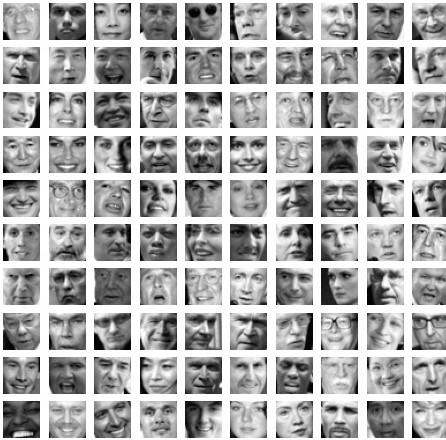
\includegraphics[scale=0.8]{faces_original.jpg}
\caption{Representação de 100 imagens do conjunto de exemplos de treinamento} \label{faces_original}
\end{center}
\end{figure}

\subsection{Determinação e Visualização das \textit{eigenfaces}}
O processo de "treinamento" \ do PCA consiste em utilizar como base do novo espaço de atributos os autovetores da matriz de covariância empírica ($\Sigma$) dos atributos que correspondam aos k maiores autovalores de $\Sigma$. 

Esse processo é realizado obtendo-se, inicialmente essa matriz de covariância através da Equação \ref{eq_sigma}. Em seguida, utiliza-se a função \textit{svd} da biblioteca \textit{numpy.linalg} para obter uma matriz (U), em que cada coluna é um dos autovetores de $\Sigma$ já ordenados com base na ordem decrescente dos autovalores correspondentes, e um vetor (S) em que cada entrada é um valor singular de $\Sigma$ obedecendo a mesma ordem da matriz de autovetores (U).

\begin{equation} \label{eq_sigma}
\Sigma = \frac{1}{m} X^tX
\end{equation}

A Figura \ref{eigenfaces} apresenta as 36 principais \textit{eigenfaces}, isto é, a representação gráfica dos 36 autovetores de $\Sigma$ cujos correspondentes autovalores são os maiores. 

\begin{figure} [htp]
\begin{center}
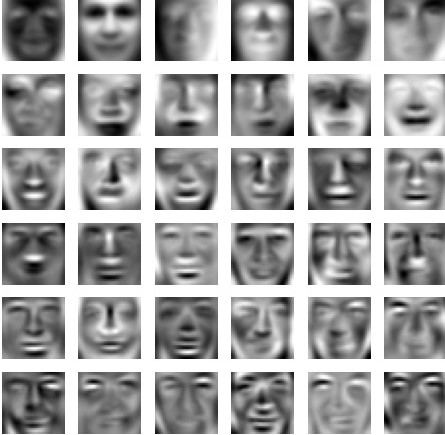
\includegraphics[scale=0.8]{eigenfaces.jpg}
\caption{Representação visual das 36 principais \textit{eigenfaces.}} \label{eigenfaces}
\end{center}
\end{figure}

É interessante observar que as \textit{eigenfaces} se parecem com imagens de faces com pouca nitidez e detalhes, o que é coerente com o que se espera, pois, com o PCA, deseja-se obter as \textit{eigenfaces} a fim de ser possível representar uma imagem de face de uma pessoa como a combinação linear de faces consideradas comuns pelo algoritmo de treinamento. 

\subsection{Projeção das Faces} \label{proj}
Uma forma útil de avaliar se de fato as \textit{eigenfaces} obtidas são boas é visualizar as faces dos exemplos de treinamento como combinação linear das \textit{eigenfaces}.

Para obter esse resultado, utilizamos as 100 principais \textit{eigenfaces} e projetamos os exemplos de treinamento sobre elas. Isso pode ser feito definindo a matriz $U_{red}$ como as 100 primeiras colunas da matriz U obtida anteriormente e definindo a projeção das imagens do conjunto de treinamento como $z=X U_{red}$. A fim de ser possível visualizar essas projeções como imagens de faces, é necessário, então, restituí-las ao espaço de atributos original, o que pode ser feito fazendo $proj = z U_{red}^t$.

As Figuras \ref{projFaces1} e \ref{projFaces2} apresentam a comparação entre as 100 faces originais e os resultados obtidos com as projeções utilizando as 100 principais \textit{eigenfaces.} Nessas figuras, as linhas ímpares apresentam as imagens originais e, abaixo, nas linhas pares, estão os resultados das projeções, a fim de facilitar a comparação. As faces utilizadas para realizar essa representação são as mesmas que as presentes na Figura \ref{faces_original}, que foram selecionadas aleatoriamente. 

\begin{figure} [htp]
\begin{center}
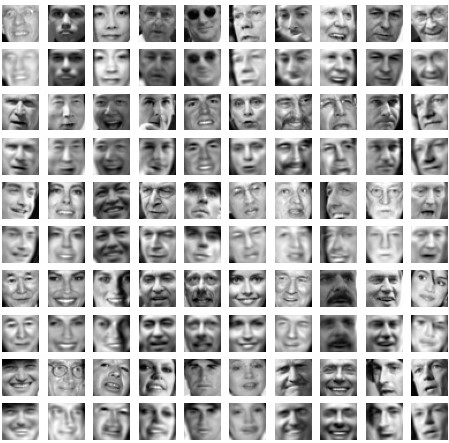
\includegraphics[scale=0.8]{projFaces1.jpg}
\caption{Comparação entre imagens originais e obtidas a partir da projeção com 100 \textit{eigenfaces.}} \label{projFaces1}
\end{center}
\end{figure} 

\begin{figure} [htp]
\begin{center}
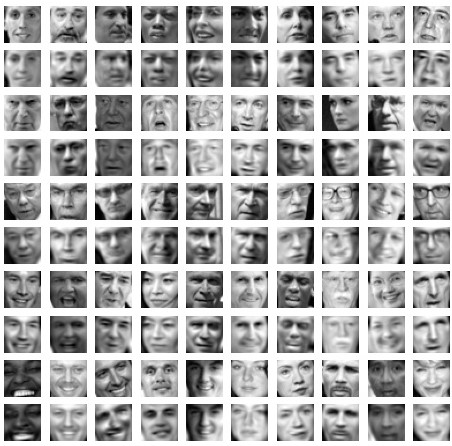
\includegraphics[scale=0.8]{projFaces2.jpg}
\caption{Comparação entre imagens originais e obtidas a partir da projeção com 100 \textit{eigenfaces.}} \label{projFaces2}
\end{center}
\end{figure} 

É interessante notar como as imagens obtidas pela projeção são similares às originais, indicando bom desempenho do processo de redução de dimensionalidade realizado. É evidente que as imagens originais apresentam mais detalhes e são mais nítidas. Contudo, as imagens originadas por projeção são bastante claras e permitem (a um humano) o reconhecimento facial das pessoas com facilidade. 

Considerando que o objetivo dessa redução de dimensionalidade é justamente possibilitar o treinamento de algoritmos de reconhecimento facial com menor custo computacional, a possibilidade de reconhecer as pessoas a partir das imagens projetas em um espaço de dimensionalidade de menos de 10\% das dimensões do espaço original é altamente significativa, devido à grande redução de custo computacional que isso implica.

É importante, todavia, ressaltar que seria necessário realizar testes sobre os algoritmos de reconhecimento facial para verificar qual é o número de componentes principais ideal que permita ao algoritmo reconhecer as faces com custo computacional adequado. A Seção \ref{var_mant} discute um pouco essa questão. 

\subsection{Fração da Variância Original Mantida} \label{var_mant}
Uma forma de medir a perda de informação gerada pelo PCA é avaliar a fração da variância original mantida. Quanto maior for essa fração, menor a perda de informação. Essa fração pode ser obtida pela equação \ref{var}, em que k é o número de componentes principais utilizado e n é o número de atributos do dado original.

\begin{equation} \label{var}
\frac{\sum_{i=1}^k S_i}{\sum_{i=1}^n S_i}
\end{equation}

A Figura \ref{variancia} apresenta um gráfico da evolução da fração da variância original mantida em função do número de componentes principais. Conforme esperado, quanto maior o número de componentes principais, maior essa fração e, portanto, menor a perda de informação. É interessante observar, contudo, como um número relativamente baixo de componentes principais já garante um valor grande dessa fração e consequente pequena perda de informação. Para k=100, por exemplo, como utilizado na Seção \ref{proj}, há cerca de 94\% da manutenção da variância original. Com 150 componentes principais, o que corresponde a pouco mais do que 10\% da dimensão original dos dados, mais de 96\% da variância original é mantida e, a partir de 350 \textit{eigenfaces}, que representa cerca de um terço do número original de atributos, já há manutenção de mais do que 99\% da variância original.

\begin{figure} [htp]
\begin{center}
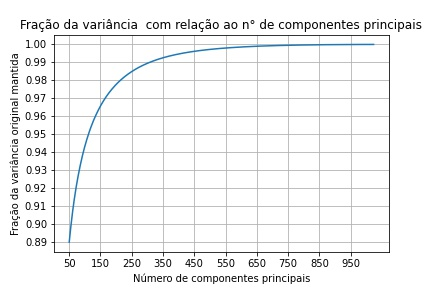
\includegraphics[scale=0.8]{variancia.jpg}
\caption{Evolução da fração da variância original mantida em relação ao número de componentes principais.} \label{variancia}
\end{center}
\end{figure}

Portanto, há grande potencial de aplicação da técnica de PCA para facilitar o treinamento de algoritmos para realização de reconhecimento facial (e de fato essa técnica é muito utilizada na prática).

\section{Referências}
Vídeo-aulas e \textit{slides} pelo Professor João Batista Florindo em ocasião de oferecimento da disciplina MS960 no segundo semestre de 2020 pelo Instituto de Matemática, Estatística e Computação Científica (IMECC) da Universidade Estadual de Campinas (UNICAMP).

\end{document}